
\chapter{The distributive property}

The distributive law will be the star of the tensor show.   Distributive laws
appear throughout our world of measurement and this offers some gentle points 
of entry to the study.  
Start with area.
\begin{center}
    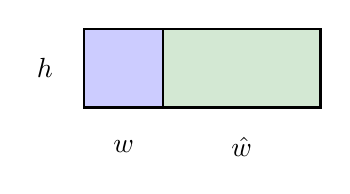
\begin{tikzpicture}
        \draw[thick, fill=blue!20] (0,0) rectangle (1,1);
        \draw[thick, fill=ForestGreen!20] (1,0) rectangle (3,1);

        \node at ( 0.5,-0.5) {$w$};
        \node at ( 2,-0.5) {$\hat{w}$};
        \node at (-0.5,0.5) {$h$};

    \end{tikzpicture}
\hspace{1in}
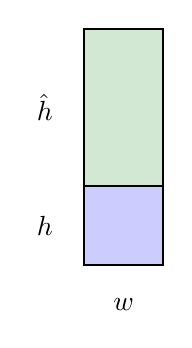
\begin{tikzpicture}
    \draw[thick, fill=blue!20] (0,0) rectangle (1,1);
    \draw[thick, fill=ForestGreen!20] (0,1) rectangle (1,3);

    \node at ( 0.5,-0.5) {$w$};
    \node at (-0.5,0.5) {$h$};
    \node at (-0.5,2) {$\hat{h}$};

\end{tikzpicture}
\end{center}
So area $A(\ell,h)$ distributes.
\begin{align*}
    A(w+\hat{w},h) &= A(w,h)+A(\hat{w},h)
    &    A(w,h+\hat{h}) &= A(w,h)+A(w,\hat{h})
\end{align*}
Used in repetition, all areas get defined by distributing measurement to 
sums of subrectangles that steadily approximate the whole.
Thus area's distributive property water-marks calculus 
in numerous ways including the following fundamental identity.
\begin{align*}
    \int_M (f+g)\text{d}x = \int_M f \text{d}x + \int_M g \text{d}x
\end{align*}

\subsection{``Real'' life}
Look elsewhere in your life.  When you buy $x$ items at cost $\text{Cost}(x)$
and then buy $y$ more the total cost is:
\[
    \text{Cost}(x+y)=\text{Cost}(x)+\text{Cost}(y).
\]  
Add the cost of tax $\text{Tax}(x)$ and the total changes to 
\[
    (\text{Cost}+\text{Tax})(x)=\text{Cost}(x)+\text{Tax}(x).
\]
Cost distributes.  

Here is another life situation.  The work of $e$ employee for $h$ hours produces 
$\text{W}(e,h)$ widgets
so at peak productivity adding $\hat{e}$ workers or $\hat{h}$ extra hours we get
\begin{align*}
    \text{W}(e+\hat{e},h)& =\text{W}(e,h)+\text{W}(\hat{e},h)
    &
    \text{W}(e,h+\hat{h})& =\text{W}(e,h)+\text{W}(e,\hat{h}).
\end{align*}
Work distributes, both over workers and over time.

Well all this is at least true for some range of values.  All scientific
claims of connection to reality are true only for sensible regions of values.

Imagine next the ingredient list 
$\text{Supplies}(r)$ of recipe $r$.  If we need to shop for ingredients of two recipes 
$r$ and $\acute{r}$ then 
\[
    \text{Supplies}(r+\acute{r})=\text{Supplies}(r)+\text{Supplies}(\acute{r}).
\]
Need to print the names of both faculty and graduate students. 
You could distribute that work as well, as seen in Listing~\ref{lst:distributive},
the command \code{Print} distributes over the operator of concatenation \code{cat}
with the result of simply appending the two individual printing commands.
We could say 
\begin{center}
    \code{Print(as cat bs) == Print(as) append Print(bs)}
\end{center}

\begin{lstfloat}
\begin{notebookin}
fac = [ "Hamilton", "Levi-Chivita" ]
students = [ TBD use math geoneolgoy to find some students of these]
Print(faculty cat students)
\end{notebookin}
\begin{notebookout}
Hamilton
Levi-Chivita
....TBD
\end{notebookout}
\begin{notebookin}
Print(faculty)
Print(students)
\end{notebookin}
\begin{notebookout}
Hamilton
Levi-Chivita
....TBD
\end{notebookout}
\caption{Many operations in computation are distributive.}\label{lst:distributive}
\end{lstfloat}

Now as a warning the purpose of these notes is to get deep into the theory and 
computation of tensors and most examples will rely on substantive mathematical 
background.  These examples however might remind you of the connections to 
concrete problems and help you communicate across the sciences and perhaps 
even to your friends and family who wonder what you do.

\subsection{Axes and valence}

By custom, area $A(\ell,w)$ of rectangle is denoted $\ell \cdot w$, called
multiplication, and the distributive law takes its form:
\begin{align*}
    (\ell+\hat{\ell})\cdot h & = \ell \cdot w +\hat{\ell}\cdot h 
    &
    \ell \cdot (h+\hat{h}) & = \ell\cdot h +\ell\cdot \hat{h}.
\end{align*}
This is the first of dozens of notations invented over the centuries to communicate 
functions that distribute their work amongst sums of sub-applications of the function.  
Most honor one of these three modes:
functions on the outside applied to sums of inputs 
\[ 
    f(u+\acute{u})=f(u)+f(\acute{u}),\qquad 
    \texttt{Print}(students+faculty),\qquad
    \text{Cost}
    (x,y,z)\ldots;
\]
functions in the middle like these operators 
\[
    (u+\acute{u})*v=u*v+\acute{u}*v, \qquad 
    (u+\acute{u})\cdot v=u\cdot v+\acute{u}\cdot v,\qquad 
    u\otimes v, \qquad 
    uv,\ldots; 
\]
or functions on the outside like these
\[
    \langle u+\acute{u}|v\rangle=\langle u|v\rangle +\langle \acute{u}|v\rangle,\qquad 
    [u+\acute{u},v]=[u,v]+[\acute{u},v],\qquad  
    /u,v/,\ldots~.
\]
   
Just, as area distributes, so does volume $V(\ell,w,h)$ only with one more axis.
\begin{center}
    \textbf{[TBD: a tikz picture of three volumes showing three axes of distributive volume]}
\end{center}
As formulas this could be written:
\begin{align*}
    V(\ell+\hat{\ell},w,h) & = V(\ell,w,h)+V(\hat{\ell},w,h)\\
        V(\ell,w+\hat{w},h) & = V(\ell,w,h)+V(\ell,\hat{w},h)\\
        V(\ell,w,h+\hat{h}) & = V(\ell,w,h)+V(\ell,w,\hat{h})
\end{align*}

Venturing into hypervolumes benefits from some notation.  For instance, the area
of a rectangle of length $\ell$ and width $w$ could be expressed  as $A(w,\ell)$
or $A(\ell,w)$ without concern because it is the letter, not its position in the
list, that conveys the meaning.  A volume of box of length $\ell$, width $w$ and
height $h$ would similarly be $V(\ell,w,h)$ or $V(h,\ell,w)$ and so on.  
We can carry this convention forward by treating inputs not as ordered lists but 
as unordered but \emph{labeled} lists.  So we have a set $A$ of axes an for each 
axis $a\in A$ the parameter in that axis is decorated by $a$, e.g.\ $x_a$.
For example $A=\{x,y\}$
Hypervolume could then be regarded as $V(x_a\mid a\in A)$.

instead of $A(x,y)$ 
because of the fixed conventions of $x$ and $y$ axes.  The letters themselves, not their position 
in the formula, are enough to understand the meaning.  With volume $V(x,y,z)$ a similar 
tolerance could be had for writing $V(z,y,x)$.  

To go further in
It 
This is one of the foundational reason for the method of calculus: we can chop area up and add the resulting smaller areas
with no affect on the result.  It's power is reflected in the final form of calculus through properties like this:
\begin{align*}
    \int_M (f+g)\text{d}x = \int_M f \text{d}x + \int_M g \text{d}x
\end{align*}


As area distributes, volume 

\section{Distributive algebra}


What does this require?
\begin{align}
    u*(v+\acute{v}) & = u*v+u*\acute{v}
    & 
    (u+\acute{u})*v & = u*v + \acute{u}*v.
\end{align}
We definitely need additions, but we should not jump to assume that $u$, $v$, and $w$ are 
of the same type.  Just look at  matrix 
multiplication (we use $\mathbb{R}^{a\times b}$ to denote $(a\times b)$-matrices 
of real numbers)
\begin{align*}
    *&:\mathbb{R}^{a\times b}\times \mathbb{R}^{b\times c}\to \mathbb{R}^{a\times c}
    &
    (u*v)_{ij} & = \sum_k u_{ik}v_{kj}.
\end{align*}
So we except this is a study of \emph{heterogeneous} algebra, so we wont be
captivated by homomorphism but rather what we will call \emph{hetero}morphisms.
So we could think of three types of data $U$, $V$ and $W$ each with a $+$ each
combined by a function 
$*:U\times V\to W$
that satisfies the distributive law.  Because this is the start it will get its own 
notation, we write $\bmto$, that is 
\begin{align*}
    *:U\times V\bmto W
\end{align*}
denotes a distributive function on additive structures $U$, $V$, and $W$.
As we go along we will prefer to use $U$, $V$ and $W$ in just this way so that 
we can get up to speed on examples as quickly as possible.


\section{Properties of addition}
It is tempting now to start  assuming that $U$, $V$, and $W$ are 
something family---vector spaces, modules, or at least abelian groups.
However this would rob the distributive law of its power and leave us to think 
addition and its common attributes are the reason tensors work.  But the 
distributive law is already claiming a strong interaction of two operations 
so maybe it should be explored on its own a little while longer to appreciate 
what it already says about the individual operations.  More examples will demonstrate 
the value of a general point of view.

We will use a number of spaces
\begin{align*}
    \mathbb{R}^d & \defeq \{u:[d]\to \mathbb{R}\},\\
    R^{m\times n} &\defeq \{M:[m]\times [n]\to \mathbb{R}\}\\
    R^{\ell\times m\times n} &\defeq \{\Gamma:[\ell]\times [m]\times [n]\to \mathbb{R}\}\\
    & \vdots
\end{align*}
Define the following operations.
\begin{gather*}
    \mathbb{R}^m\oplus \mathbb{R}^n  \defeq \mathbb{R}^{m+n}\\
    \begin{bmatrix} \mathbb{R}^{a\times n} \\ \mathbb{R}^{b\times n} \end{bmatrix} \defeq \mathbb{R}^{(a+b)\times n}
    \qquad
    \begin{bmatrix}
    \mathbb{R}^{m\times c} &
    \mathbb{R}^{m\times d}
    \end{bmatrix}  \defeq \mathbb{R}^{m\times (c+d)}\\
%     \mathbb{R}^{a\times m\times n} \oplus \mathbb{R}^{b\times m\times n}  \defeq \mathbb{R}^{(a+b)\times m\times n}
%     \qquad
%     \mathbb{R}^{\ell \times c\times n} \oplus \mathbb{R}^{\ell \times d\times n}  \defeq \mathbb{R}^{\ell\times (c+d)\times n}
%     \qquad
% \\  
%      \mathbb{R}^{\ell \times m\times e} \oplus \mathbb{R}^{\ell \times m\times f}  \defeq \mathbb{R}^{\ell\times m\times (e+f)}\\
     \vdots
\end{gather*}



Now we add a multiplication.
\begin{align*}
    \mathbb{R}^m \otimes \mathbb{R}^n & \defeq \mathbb{R}^{m\times n}
\end{align*}

\begin{example}
    The distributive law with vector space operators.
    \begin{align*}
    (\mathbb{R}^a \oplus \mathbb{R}^b)\otimes \mathbb{R}^n 
        % & = \mathbb{R}^{(a+b)\times c}
        &  = \begin{bmatrix}\mathbb{R}^{a}\otimes \mathbb{R}^n  \\ \mathbb{R}^b\otimes \mathbb{R}^n\end{bmatrix}\\
    \mathbb{R}^m\oplus ( \mathbb{R}^c \oplus \mathbb{R}^d )
        % & = \mathbb{R}^{(a+b)\times c}
        &  = \begin{bmatrix} 
            \mathbb{R}^{m}\otimes \mathbb{R}^c &
            \mathbb{R}^m\otimes \mathbb{R}^d
        \end{bmatrix}
    \end{align*}
\end{example}

Lets combine the left and right 
distributive laws.

\begin{center}
    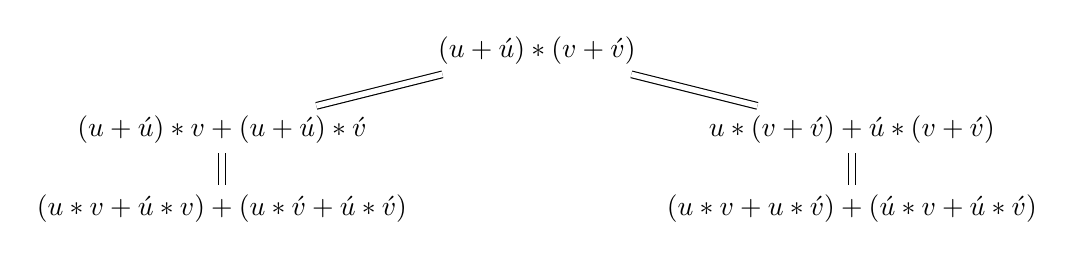
\begin{tikzpicture}[xscale=2]
        \node (A) at (0,0) {$(u+\acute{u})*(v+\acute{v})$};
        \node (B) at (-2,-1) {$(u+\acute{u})*v+(u+\acute{u})*\acute{v}$};
        \node (C) at (2,-1) {$u*(v+\acute{v})+\acute{u}*(v+\acute{v})$};
        \node (D) at (-2,-2) {$(u*v+\acute{u}*v)+(u*\acute{v}+\acute{u}*\acute{v})$};
        \node (E) at (2,-2) {$(u*v+u*\acute{v})+(\acute{u}*v+\acute{u}*\acute{v})$};
        \draw[double distance=2pt] (A) -- (B);
        \draw[double distance=2pt] (A) -- (C);
        \draw[double distance=2pt] (B) -- (D);
        \draw[double distance=2pt] (C) -- (E);
    \end{tikzpicture}
\end{center}
Thus the values $a,b,c,d,\ldots $ in the image of a distributive product $*:U\times V\bmto W$ must 
satisfy the following identity.
\begin{equation}
    \tag{Distributable}
    (a+b)+(c+d) = (a+c)+(b+d)
\end{equation}

\begin{proposition}
    If $+$ in both associative and commutative then it is distributable.

    Conversely, if $+$ is 
\end{proposition}